相较于直接测量浓度,通过分析手段得到与一个浓度成比例的仪器信号在操作上更为便捷。此类仪器信号包括吸光度、荧光强度和电导率等。这种方法的要求是,反应物和产物都能给出与其浓度直接成正比的信号,且该能被观察到的性质在反应过程中有实验上可用的变化。在下述实验中,可以使用吸收光谱和比尔定律。

\textbf{A}是反应物,\textbf{B}是唯一产物(\textbf{A}$\rightarrow$\textbf{B}),两者在指定波长下均有吸收,且吸光度与其浓度成正比。在此实验中,$\varepsilon_A\neq\varepsilon_B$,其中$\varepsilon$是摩尔吸光系数。

下表给出在水溶液中\textbf{A}水解为\textbf{B}时的吸光度数据。实验条件为:pH为中性即7.0,温度是25 °C,\textbf{A}的初始浓度为4.0 × 10\textsuperscript{--6} M,使用吸收波长400 nm和5 cm吸收皿。

\begin{longtable}[]{@{}llllllll@{}}
	\toprule
	\emph{t}/s &0&20&60&120&160&200&$\infty$ \tabularnewline
	A\textsubscript{t} & 0.0840&0.1090&0.1515&0.2010&0.2255&0.2440&0.3170\tabularnewline
	\bottomrule
\end{longtable}

\noindent\textbf{23.1.}计算在题给条件下\textbf{A}和\textbf{B}的摩尔吸光系数。

\noindent\textbf{23.2.}计算反应速率常数。

\noindent\textbf{23.3.}计算反应半衰期(\emph{t}\textsubscript{1/2})。

\noindent\textbf{23.4.}计算在多少秒后{[}\textbf{A}{]}变为1.0×10\textsuperscript{-6}
M?

\noindent\textbf{23.5.}如果30 ℃时$k$ = 0.01029 s\textsuperscript{-1},计算$E_a$。

\noindent\textbf{23.6.}假设过渡态速率常数与由实验数据得到的结果相同,计算活化自由能。

$$
k_{\mathrm{TST}} =\frac{k_BT}{h}e^{-\Delta G^\ddag/RT}
$$

\noindent 其中$k_B$是玻尔兹曼常数,$h$是普朗克常数,$R$是理想气体常数。

酸催化下乙二醇和对苯二甲酸的缩合反应的速率是反应进度(即{[}\textbf{A}{]}与{[}\textbf{A}{]}\textsubscript{0}之比)的函数,该反应遵循二级反应动力学。两个单体的浓度相等,均为{[}\textbf{A}{]}\textsubscript{0} = 4.8 mol dm\textsuperscript{-3}。

\begin{figure}[h]
	\centering
	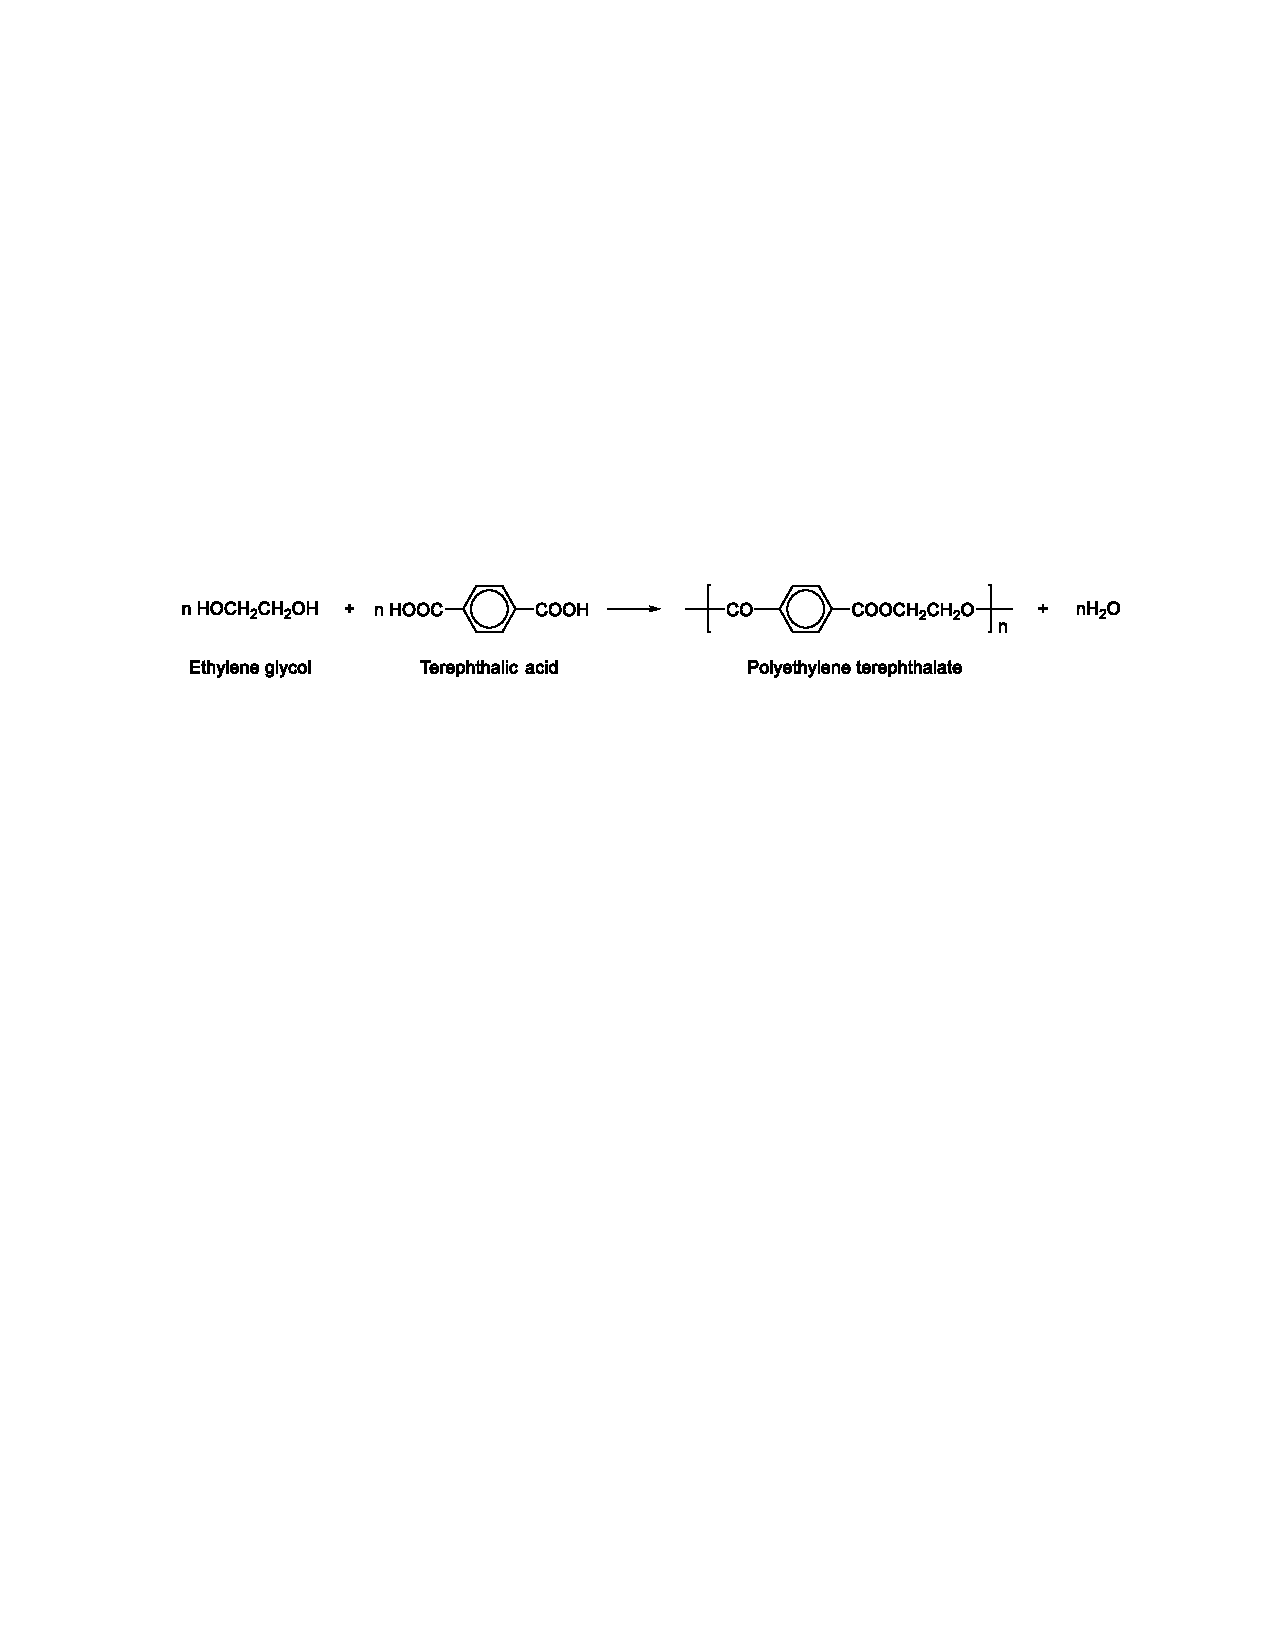
\includegraphics[width=15cm]{./pic/t23-1.pdf}
\end{figure}

\begin{longtable}[]{@{}lllll@{}}
\toprule
时间(h) &0&0.5&1.5&2.5 \tabularnewline
反应进度 & 0&0.636&0.839&0.897\tabularnewline
\bottomrule
\end{longtable}

\noindent\textbf{23.7.}计算速率常数。

\noindent\textbf{23.8.}计算反应半衰期。

\noindent\textbf{23.9.}一小时后单体的浓度为多少?
